\chapter{Experiments}
\label{ch:Experiments}

In this chapter, we compare the runtimes of three summation modes:
The Binary Tree Summation algorithm as presented in \Cref{ch:BinaryTreeSummation} and \Cref{ch:Implementation}, the ReproBLAS reduce operation and additionally, a bitwise-irreproducible implementation which uses \texttt{std::accumulate} to sum values locally and \texttt{MPI\_Allreduce} for global reduction, as baseline.

\section{Experimental Setup}
\label{sec:ExperimentalSetup}
We ran shared-memory benchmarks on a machine with two AMD EPYC 7713 CPUs with $64$ cores each for a total of $p=256$ \glspl{pe} with hyper-threading.
Distributed-memory benchmarks with more than $256$ \glspl{pe} were executed on multiple thin nodes of the bwUniCluster 2.0 which have two Intel Xeon Gold 6230  with $40$ cores ($80$ threads) per node.


\begin{table}
\centering
\caption{Overview of benchmark datasets}
\label{table:datasets}
\begin{tabular}{r|l}
\textbf{dataset name} & \textbf{number of summands $N$} \\
\hline
354 & $460$ \\
multi100 & $767$ \\
prim & $898$ \\
fusob & $1\,602$ \\
dna\_rokasD4 & $239\,763$ \\
aa\_rokasA8 & $504\,850$ \\
dna\_rokasD1 & $1\,327\,505$ \\
aa\_rokasA4 & $1\,806\,035$ \\
dna\_PeteD8 & $3\,011\,099$ \\
dna\_rokasD7 & $21\,410\,970$ \\
\end{tabular}
\end{table}

Input data stems from RAxML-NG runs in the form of an array of double-precision floating point numbers representing per-site log-likelihood values.
Dataset sizes range from $460$ to $21\,410\,970$ elements, as listed by \Cref{table:datasets}.

The benchmark execution performs the following steps for each summation mode (\texttt{reproblas}, \texttt{allreduce}, \texttt{tree}) and each dataset:
First, it loads the input data from a file and distributes it among the \glspl{pe}.
Next, it performs the summation $100$ times and measures the duration for each iteration.
Finally, it discards the first and last eight measurements and outputs both the summation result and the remaining measurements.

\section{Results}
\label{sec:Results}

\begin{figure}
\begin{subfigure}{0.49\textwidth}
\centering
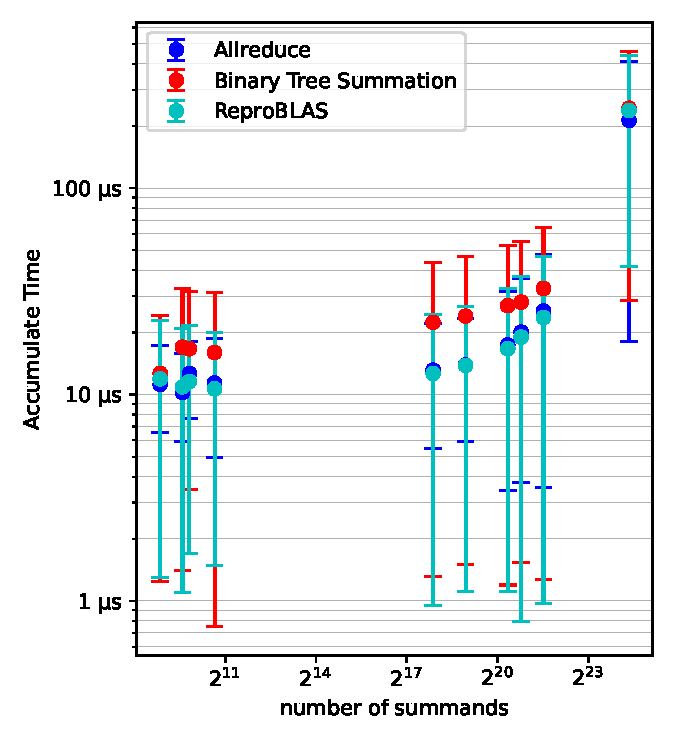
\includegraphics[scale=0.72]{figures/benchmarkScatter.pdf}
\caption{Shared memory, $p=256$}
\label{fig:benchmarkOverview256}
\end{subfigure}
\hfill
\begin{subfigure}{0.49\textwidth}
\centering
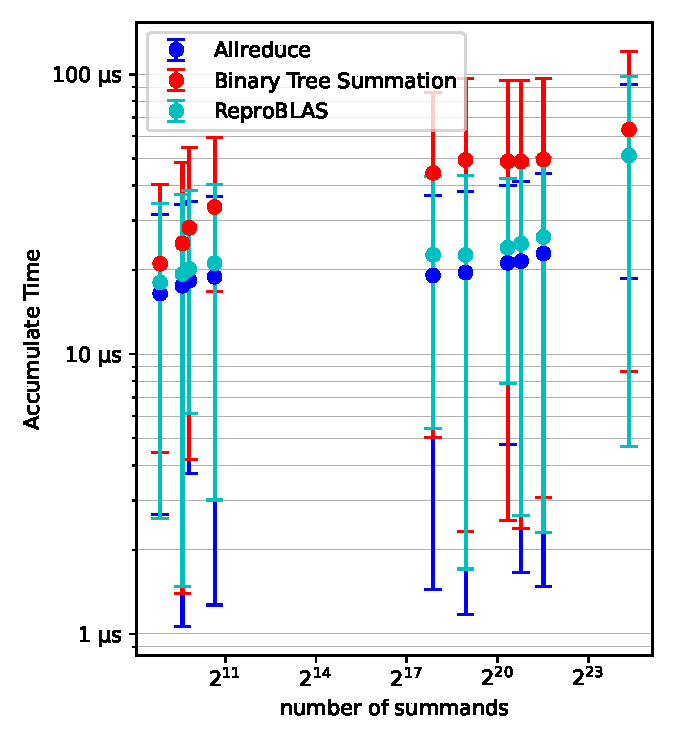
\includegraphics[scale=0.72]{figures/benchmarkScatter1280.pdf}
\caption{Distributed memory, $p=1280$}
\label{fig:benchmarkOverview1280}
\end{subfigure}

\caption{Median accumulation time after 100 repetitions for different datasets. Error bars depict 1st and 99th percentile.}
\label{fig:benchmarkOverview}
\end{figure}

\begin{figure}
\centering
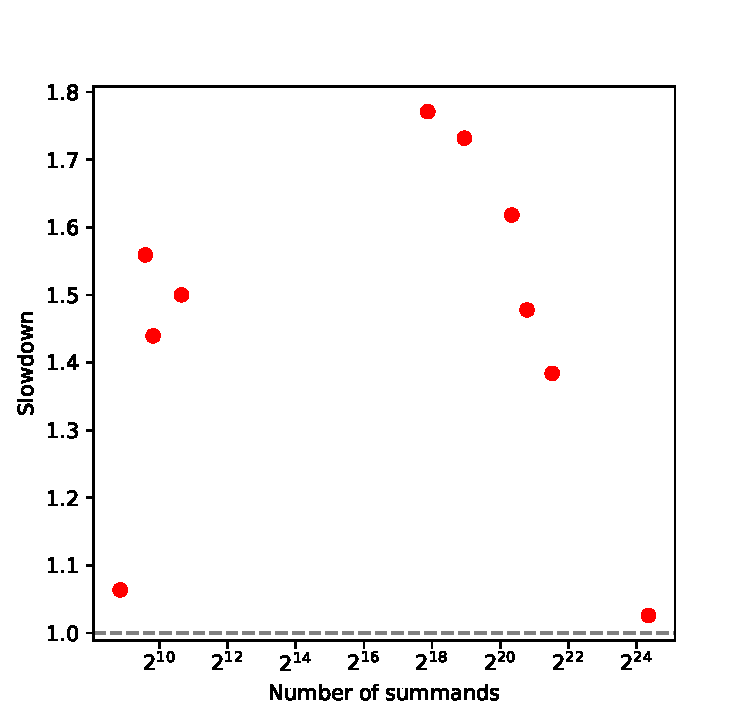
\includegraphics[scale=0.75]{figures/slowdownPlot.pdf}
\caption{Relative slowdown of Binary Tree Summation compared to ReproBLAS for $p=256$ \glspl{pe}}
\label{fig:slowdownPlot}
\end{figure}

\Cref{fig:benchmarkOverview} shows the runtime measurements across all datasets as a scatter plot.
We measure that all summation algorithms have a runtime that is linear in the number of summands (\Cref{fig:benchmarkOverview}).
On the shared-memory machine, we measure a slowdown of less than $2$ of Binary Tree Summation compared to ReproBLAS (\Cref{fig:slowdownPlot}).
On the largest dataset, Binary Tree Summation is only $2\,\%$ slower than ReproBLAS (\Cref{fig:boxplotRokasD7}).
The runtime of the irreproducible \texttt{std::accumulate} + Allreduce variant differs less than $15\,\%$ from the ReproBLAS runtime, possibly due to the missing vectorization of \texttt{std::accumulate} (\Cref{fig:slowdownAllreduceReproblas}).
The performance of all three accumulation modes suffers from the increased number of \glspl{pe} on the distributed-memory machine for small- and medium-sized datasets, as we observe no speedup for $N < 2^{22}$.
Additionally, the logarithmically increasing message count of Binary Tree Summation further increases the gap to ReproBLAS for increasing \gls{pe}-counts.\@

\begin{figure}
\centering
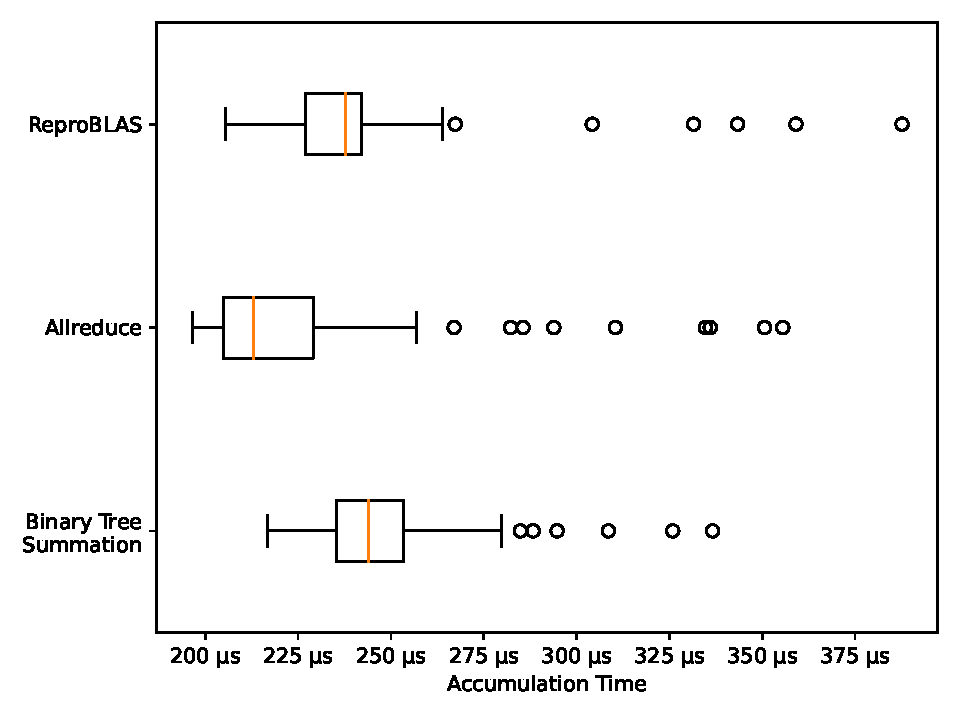
\includegraphics[scale=0.75]{figures/boxplotRokasD7.pdf}
\caption{Runtime distribution for all three summation modes on the dataset \textit{rokasD7} ($N = 21\,410\,970, p = 256$). The lowest and highest outlier removed for each accumulation mode.}
\label{fig:boxplotRokasD7}
\end{figure}


\section{Reproducibility of Results}
\label{sec:VerificationOfReproducibility}
To verify the reproducibility of the results, we ran all three summation algorithms with different core-counts in steps of 16 ($p \in \{1, 17, \ldots, 241 \}$).
With ReproBLAS and Binary Tree Summation, we detected no deviation between results for all test datasets, while values produced by Allreduce were already  irreproducible between runs with $p=1$ and $p=17$ \glspl{pe}.
\Cref{table:runDeviation} shows the difference between the largest and smallest result collected over all values of $p$.
For ReproBLAS and Binary Tree Summation, this value is zero,\footnote{Or at least smaller than the machine epsilon for IEEE 754 double precision floating-point numbers} indicating that the result is independent from the number of \glspl{pe}.
For Allreduce, the largest observed relative error was $3.9 * 10^{-13}$ (dataset \textit{rokasD1}), which could potentially cause tools like RAxML-NG to dismiss certain trees during likelihood maximization and produce different results depending on the core-count.
Results from ReproBLAS and Binary Tree Summation were also reproducible across different machines and compiler versions.\footnote{Linux 5.4.0-89-generic with GCC 9.4.0 on i10pc138, Linux 4.18.0-193.65.2.el8\_2.x86\_64 with GCC 11.2 on bwUniCluster 2.0}

\begin{table}
\centering
\begin{tabular}{llll}
\textbf{Dataset} & \textbf{ReproBLAS }& \textbf{Binary Tree Summation} & \texttt{std::accumulate}\textbf{ + AllReduce} \\
multi100 & $$0.0$$ & $0.0$ & $3.6 * 10^{-12}$ \\
rokasD1 & $0.0$ & $0.0$ & $4.5 * 10^{-6}$ \\
rokasA8 & $0.0$ & $0.0$ & $4.5 * 10^{-8}$ \\
fusob & $0.0$ & $0.0$ & $4.5 * 10^{-11}$ \\
PeteD8 & $0.0$ & $0.0$ & $6.1 * 10^{-6}$ \\
rokasD4 & $0.0$ & $0.0$ & $1.9 * 10^{-7}$ \\
rokasA8 & $0.0$ & $0.0$ & $2.8 * 10^{-6}$ \\
354 & $0.0$ & $0.0$ & $6.4 * 10^{-12}$ \\
prim & $0.0$ & $0.0$ & $7.3 * 10^{-12}$
\end{tabular}
\caption{Difference between smallest and largest obtained sum from runs with varying \gls{pe}-count}
\label{table:runDeviation}
\end{table}

\begin{figure}
\centering
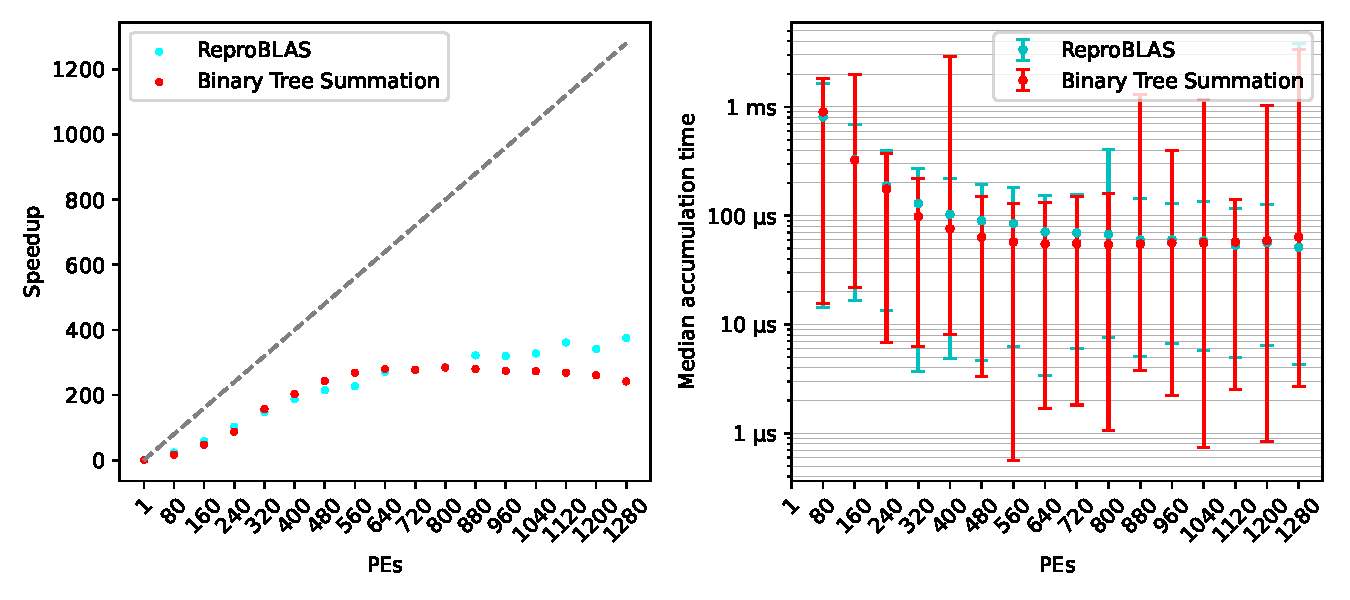
\includegraphics[scale=0.72]{figures/scaling.pdf}
\caption{Speedup and median accumulation time of $N=21\,410\,970$ elements over $p$. Error bars depict 1st and 99th percentile.}
\label{fig:ClusterScaling}
\end{figure}


\Cref{fig:ClusterScaling} shows the result of a strong-scaling benchmark on a distributed-memory machine.
The speedup relative to the sequential computation levels off for $p \geq 640$ (about $33\,000$ elements per \gls{pe}) for both ReproBLAS and Binary Tree Summation.
Between $320$ and $880$ \glspl{pe} the median accumulation time of Binary Tree Summation is smaller compared to ReproBLAS, but has a higher variance of runtimes.
